%
% Chapter 4
%

\chapter{PHYSICS OBJECTS}
Each of the CMS subdetectors (neglecting the trigger system) technically only record and detect hits and energy deposits. While these hits and energy deposits are almost
always due to passing particles, the detectors themselves and more precisely the readouts, only produce information about the position, value, and multiplicity of
these hits and energy deposits. It is thanks to clever and accurate experimental techniques that we can reconstruct various particles from these hits and energy deposits.
In part because CMS does not detect particles directly, reconstructed particles are referred to as physics \emp{objects} in this context. Using
the term particles implies certainty about the identify of the object, and because there is some uncertainty, however small, inherent in the reconstruction, objects is
more accurate and widely used. The reconstruction technique varies greatly with different objects and the subdetectors used to detect and record their hits and energy
deposits. 

\section{Object Reconstruction and Particle Flow}
The particle flow algorithm is used by CMS to reconstruct physics objects from hits and energy deposits. Particle Flow and CMS are unique in the sense
that nearly all physics analyses performed on data collected by CMS use objects reconstructed with this single algorithm. The primary advantage of this strategy is
uniform and consistent object definitions across nearly all papers published on behalf of CMS. Other collaborations such as ATLAS do not use
the same algorithm collaboration-wide. The purpose of particle flow is to identify all final-state stable particles in an event recorded by CMS, specifically electrons,
mouons, taus, jets and photons. Particle flow optimally combines building-block information (hits and energy clusters) from all subdetectors to reconstruct objects and
determine particle type, position, and momentum. It does this using 2 different primary reconstruction techniques for reconstructing tracks from tracker hits, and clusters
of energy deposits from individual calorimeter cells. 

\begin{figure}[hbtp]
 \begin{center}
   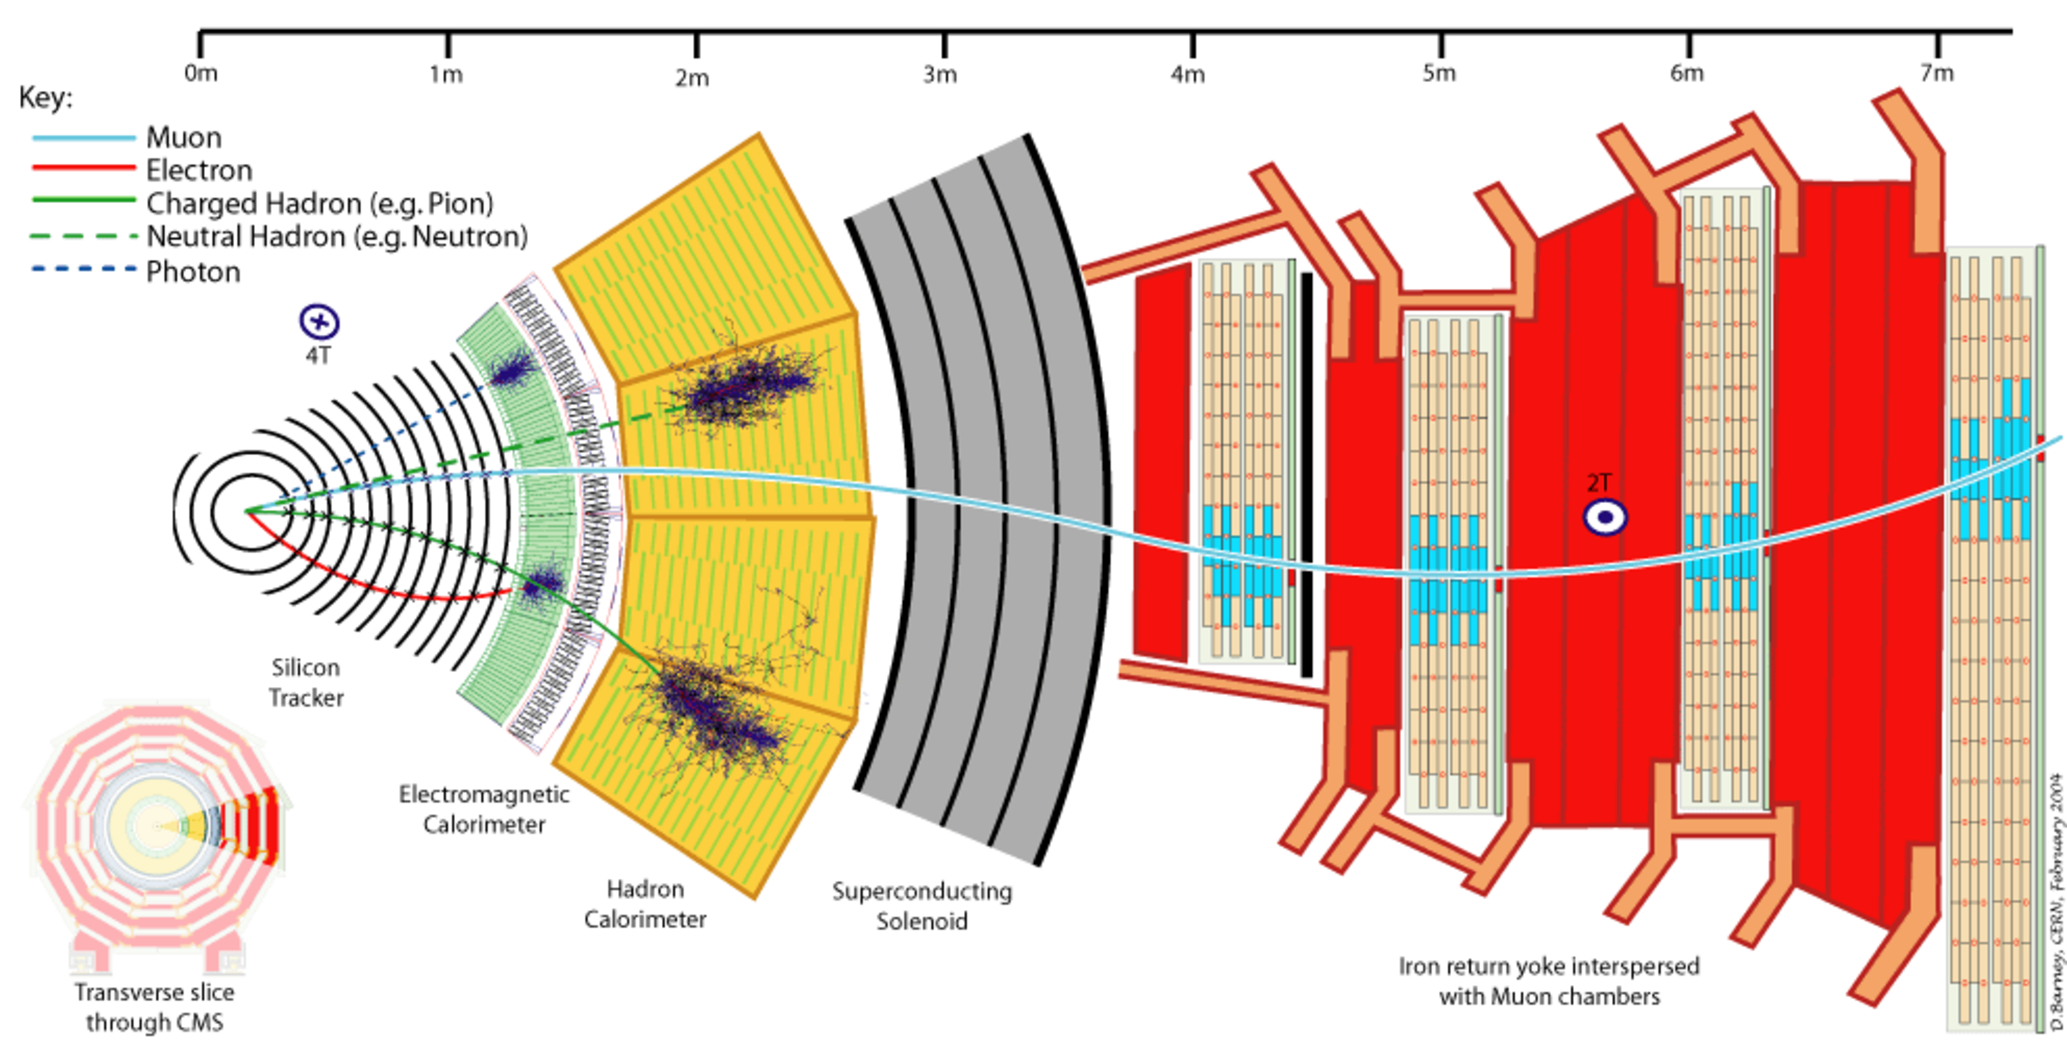
\includegraphics[width=0.8\textwidth]{ch4_figs/cms_particleflow.pdf}
   \caption{An overview of how CMS detects different types of particles. The slice of CMS in in the x-y plane.~\cite{cms_pflow_img}.}
   \label{fig:cms_pflow}
 \end{center}
\end{figure}

Object reconstruction begins with grouping collections of hits into tracks in an iterative process~\cite{CMS-TRK-09-001}. In the first iteration, tracks are
seeded with initial hits and subject to very tight criteria, sacrificing efficiency for a low fake rate. In the following iterations, hits assigned to
tracks in the previous iteration are removed from further consideration, and the criteria for candidate tracks is gradually relaxed with each iteration. In the final iterations,
the constraints on the track seed are relaxed to account for secondary decays from photon conversions and nuclear interactions with the silicon tracker material. This technique
reconstructs tracks with as few as three hits and \pts as small as 150 MeV with a fake rate in the single digits~\cite{CMS-PFT-09-001}. A similar but separate track
reconstruction is performed in the muon chambers to reconstruct muon tracks. 

Object reconstruction continues in the calorimeters, where it relies on a clustering algorithm to identify individual energy deposits and associate them to an object. This
algorithm is designed to yield a high efficiency even for low energy, and nearby objects. The clustering process is performed separately in the ECAL and HCAL, and furthermore in
the barrel, and endcaps. The ECAL preshower also uses separate clusterings in each of its two layers. In the HF, no clustering is performed, where each module is considered an
independent cluster. The clustering algorithm begins by identifying cells (cluster seeds) with an energy above a given ``seed'' energy threshold. Clusters are then increased by
adding adjacent\footnote{sharing at least one edge with the seed} cells that have an energy above a given threshold. The calorimeter granularity is used to optimize the
determination of cluster energies and positions~\cite{CMS-PFT-09-001}.  

After the tracking and clustering is complete, Particle Flow then matches tracks in the tracker to energy clusters in the calorimeters, and to tracks in the muon chambers.
In a given event, there can be many different objects and Particle Flow utilizes
a process-of-elimination strategy. Because they are the easiest to identify unambiguously, muons are identified first by matching tracks in the inner tracker to the tracks in
the muon chambers. The matching criteria is based on a $\chi^{2}$ fit threshold. When multiple sets of tracks are matched, the set with the lowest $\chi^{2}$ is selected as the
muon object. Muons are first reconstructed this way and called global muons. Particle flow muons are identifed from global muons when the \pt~s measured in the tracker and the
muon chambers agree to within three standard deviations. The tracks corresponding to the muon object are then removed from consideration for the remaining object reconstruction. 

Following muons, electrons are reconstructed next. Because electrons deflect strongly in the magnetic field, they leave characteristically short tracks, and lose energy via
Bremsstrahlung radiation. The tracks are flagged based on these characteristics as potential electron candidates and refitted with a Gaussian-Sum Filter (GSF)~\cite{gsf} and the
resulting tracks are then matched to ECAL energy clusters. The Bremsstrahlung photons are emitted tangentially to electron track and this is accounted for in the ECAL clustering
and track matching specifically for electrons. These matches are then subject to additional quality criteria before they are considered particle flow electrons, and their
corresponding tracks and energy deposits removed from further consideration for the remaining object reconstruction. 

At this point in the event/object reconstruction, the so-called low lying fruit has been picked, and the more difficult objects are all that remain. These objects are charged
and neutral hadrons (jets), and photons. The neutral particles are difficult to reconstruct because they don't leave hits in the tracker, so only calorimeter information is
available. Photons are distinguished from neutral hadrons by separate ECAL and HCAL clusters. Photons interact with and are stopped by the ECAL, while the same is true for
neutral hadrons and the HCAL. Additional in-event calibration techniques are also used to further distinguish these objects. The remainig tracks are subject to tighter
quality cuts aimed at reducing the fake-rate. The high-quality tracks passing these thresholds are matched to ECAL and HCAL deposits, and give rise to particle flow 
charge hadrons. The momentum of these objects is measured from the track radius and compared to the corresponding energy deposit in the calorimeters assuming the object is
a charged pion. If the two measurements are compatible, the momenta is refined with additonal fits to the tracks and energy deposit(s)~\cite{CMS-PFT-09-001}.

The charged and neutral hadron objects with tracks and matched energy deposits are only considered particle flow candidates at this stage.
An additional clustering step is necessary to reconstruct jet objects. As mentioned previously, when free quarks produced in the pp collision decay in the
fragmentation/hadronization process, they produce energetic and collimated sprays of charged
and neutral hadrons, called jets. To accurately determine the direction and momentum of the initial quark, as many of the corresponding charged and neutral hadrons as possible must not only be
reconstructed correctly and identified, but also clustered together (matched) correctly.
These jets are then intrepreted experimentally to be the free quark. An depiction of the hadronization and jet detection process is below in Figure~\ref{fig:frag}.

\begin{figure}[hbtp]
 \begin{center}
   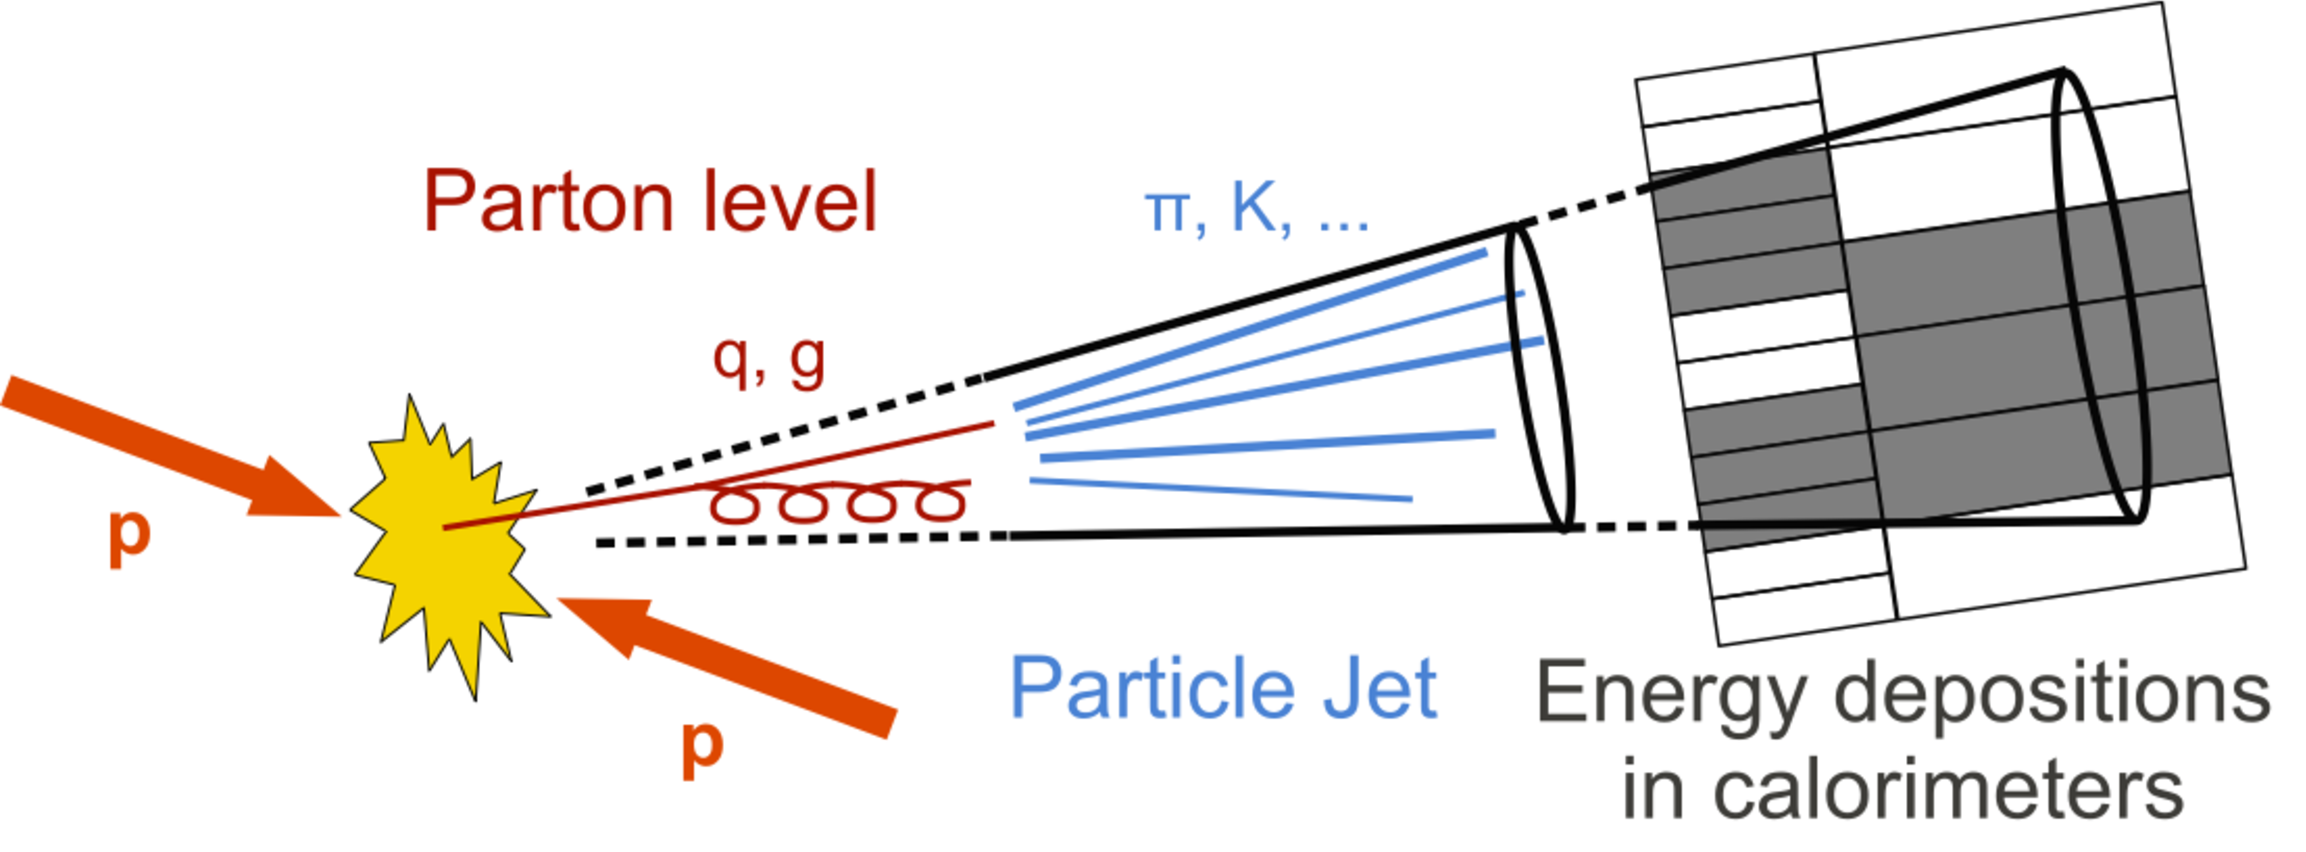
\includegraphics[width=0.8\textwidth]{ch4_figs/jet_frag.pdf}
   \caption{An example of quark hadronization and the resulting jet.~\cite{frag}.}
   \label{fig:frag}
 \end{center}
\end{figure}
 
Unfortunately, there are too many PF candidates detected and reconstructed in the calorimeters in a given event at one time to make the jet clustering process straight-forward
and unambiguous. To address this, jet clustering algorithms are used for clustering. These algorithms exploit information from the detector with theoretical knowledge of the
hadronization process to cluster the jets sensible and reproducible manner.
While many clustering algorithms exist, the one used by this analysis is the anti-$k_{T}$ algorithm~\cite{antikt}. Anti-$k_{T}$ begins like other sequential clustering algorithms,
by calculating the distance measures in equations~\ref{eqn:antikt1}. 

\begin{equation}
\begin{aligned}
\label{eqn:antikt1}
%%\begin{split}
d_{ij} &= min(k^{2p}_{Ti},k^{2p}_{Tj})\frac{\Delta_{ij}^{2}}{R^{2}} \\ d_{iB} &= k^{2p}_{Ti}
%%\end{split}  
\end{aligned} 
\end{equation}

\noindent where $\Delta_{ij}^{2} = (y_{i}-y_{j})^{2} + (\phi_{i}-\phi_{j})^{2}$ and $y_{i}$,$k_{Ti}$ are the rapidity and momenta of particle i respectively. After the
distance measures have been calculated for each candidate in the event, the smallest $d_{ij}$ are merged into one object by summing the 4-momenta of particles i and j, the
distance measures are updated and the algorithm moves onto the next smallest $d_{ij}$. If a particle has the smallest $d_{iB}$, it is removed and called a jet. This
iterative process continues until all PF candidates are clustered into jets. What differentiates anti-$k_{T}$ from Cambridge-Aachen and other similar algoirthms is the choice
of p = -1 in equation~\ref{eqn:antikt1}. This negative value explains the name of the algorithm, and the tendancy for it to produce circular\footnote{circular in the
$\eta$-$\phi$ plane} jets, centered on the highest \pt~candidate of the jet. The effect of these parameter values with respect to other available algorithms is below in
Figure~\ref{fig:jet_cluster}.

\begin{figure}[htbp] 
  {\centering
    \subfigure[$k_{T}$]{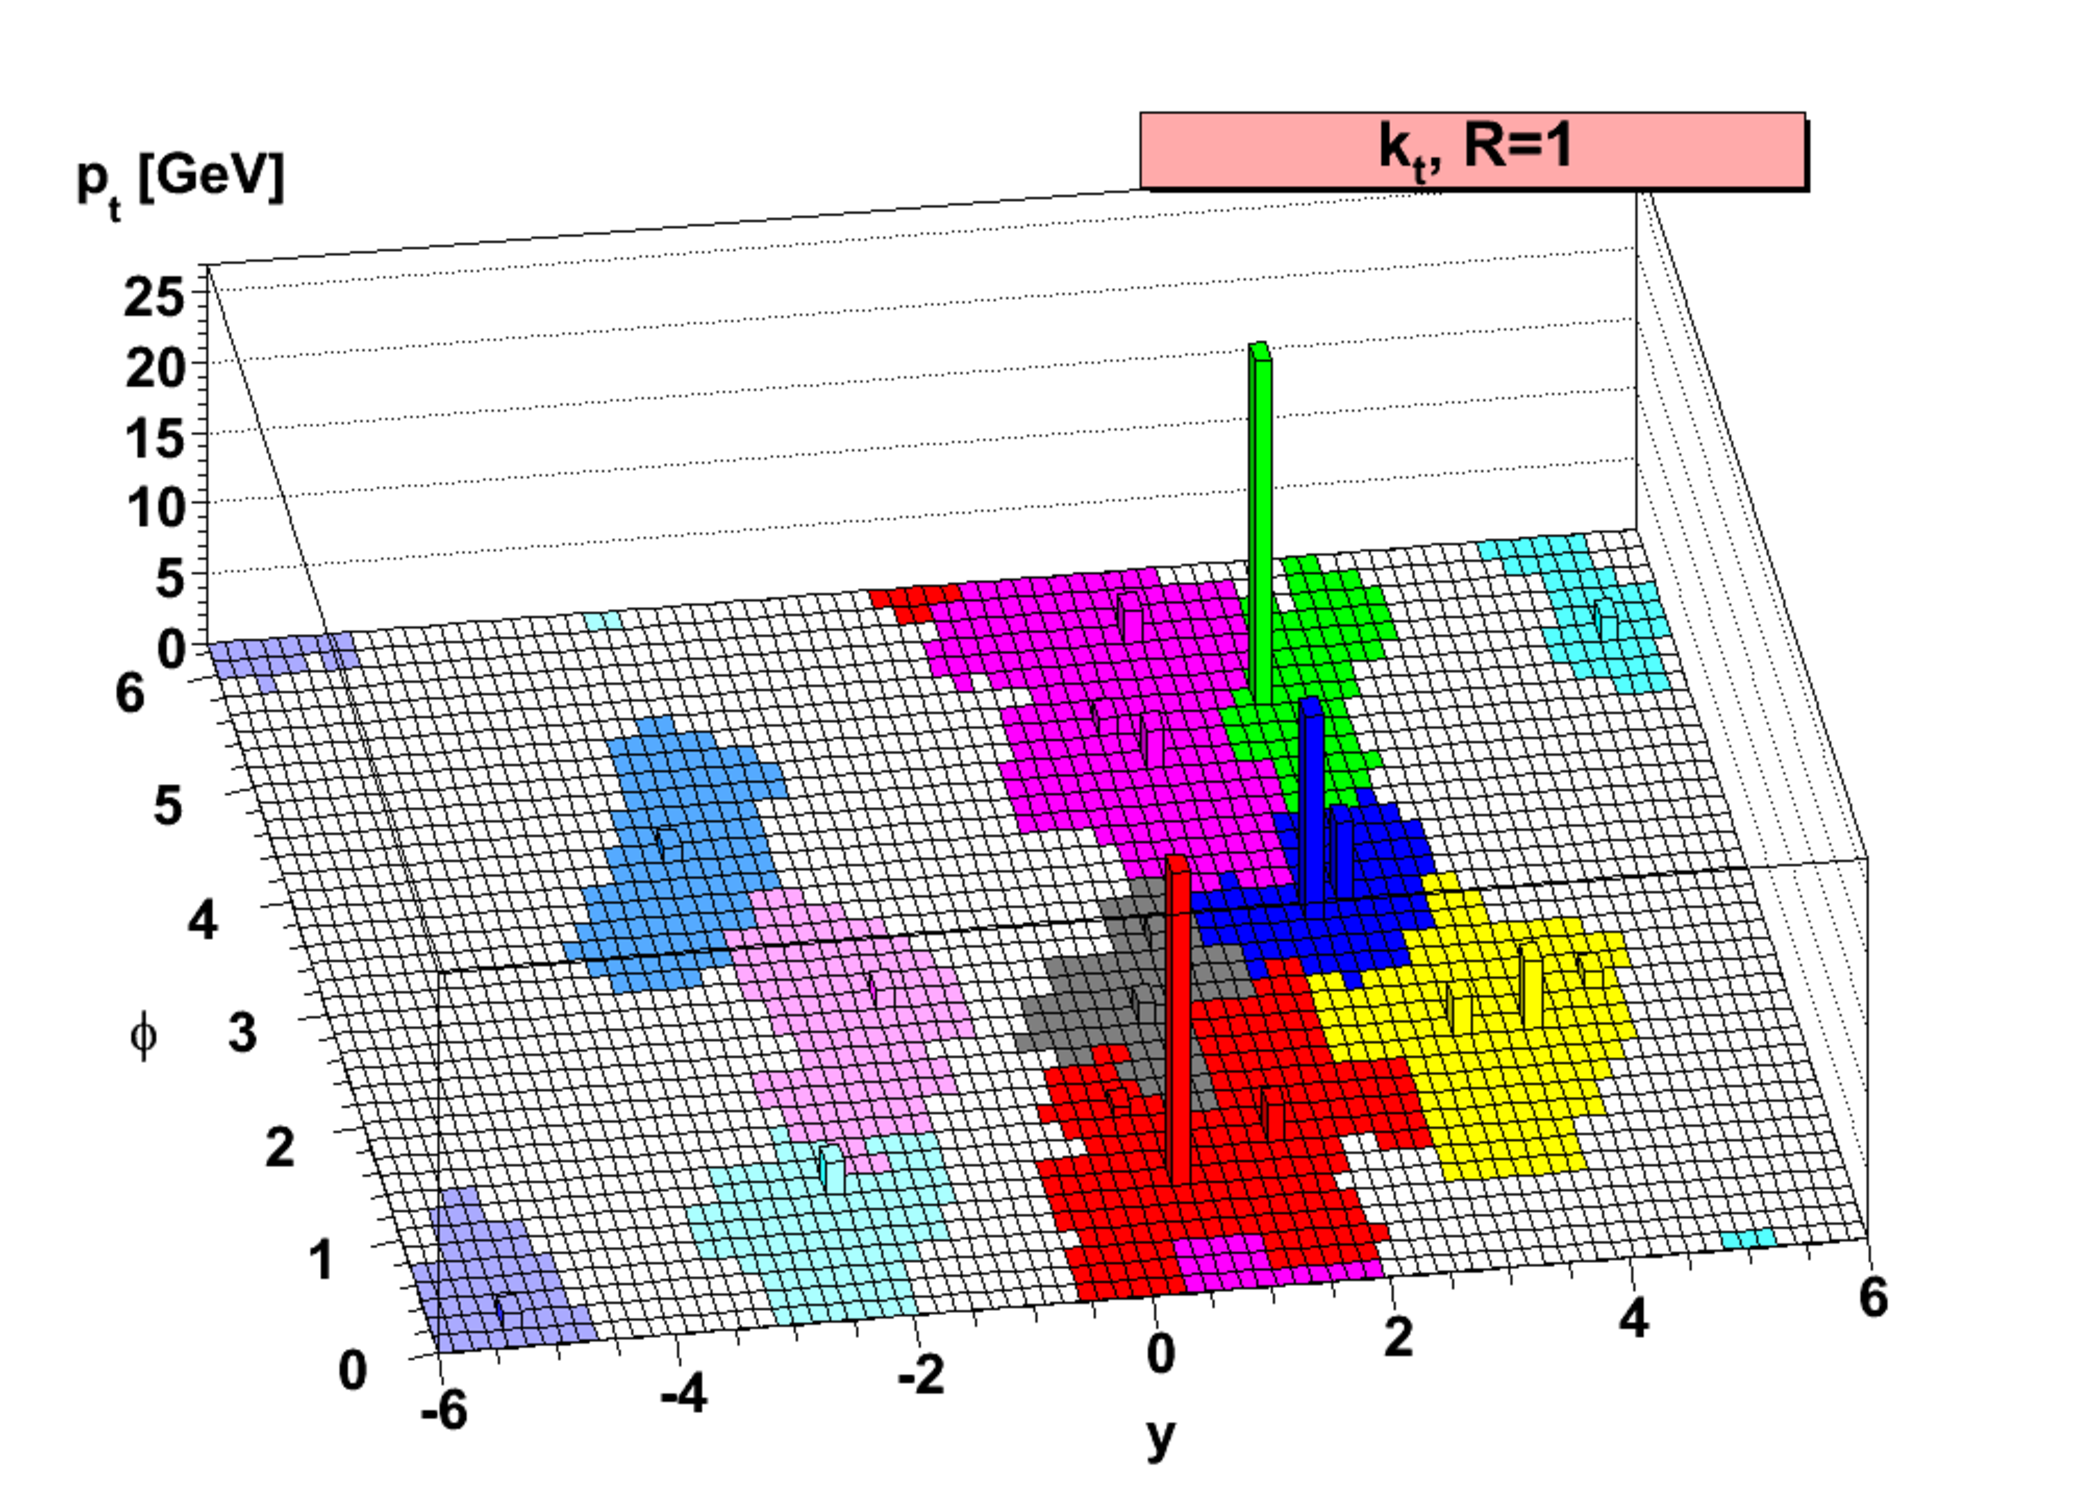
\includegraphics[width=0.4\textwidth]{ch4_figs/kt.pdf}}
    \subfigure[Cambridge-Aachen]{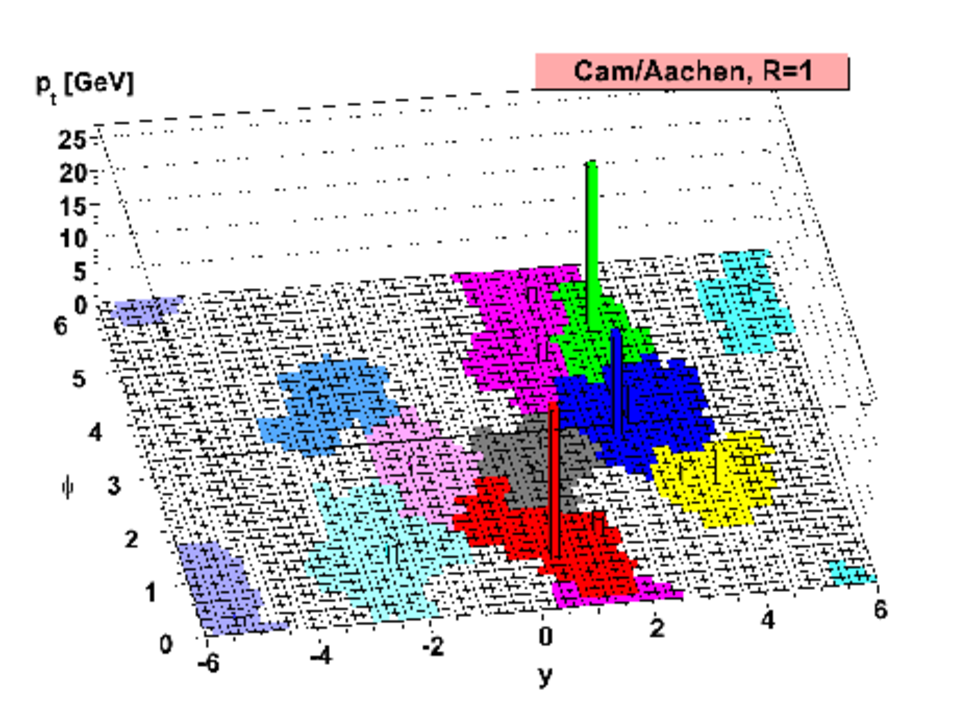
\includegraphics[width=0.4\textwidth]{ch4_figs/ca.pdf}}
    \subfigure[SIScone]{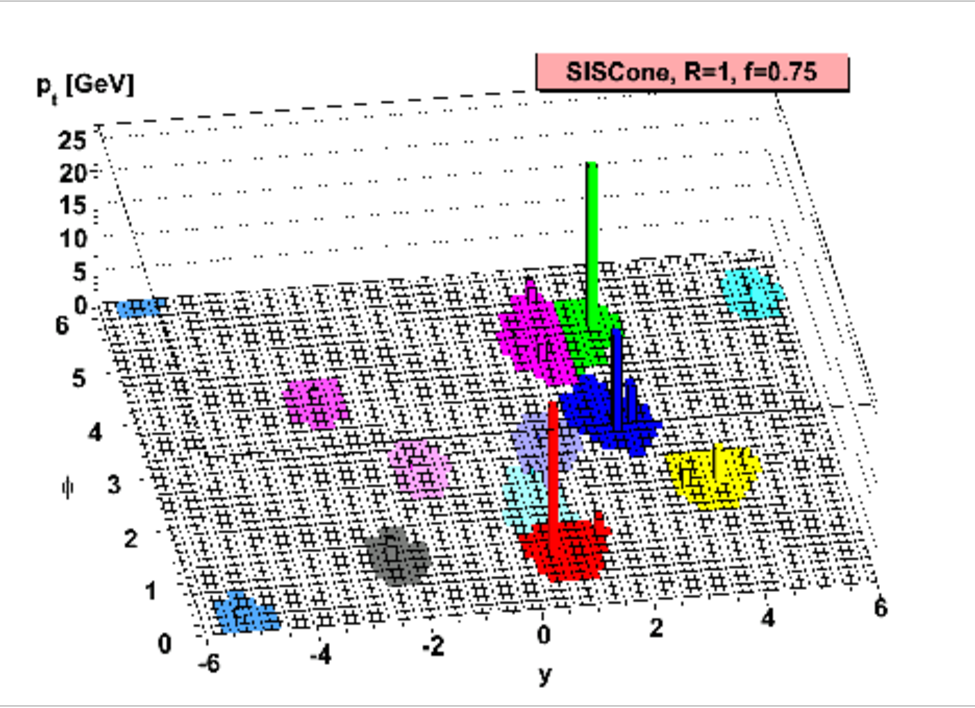
\includegraphics[width=0.4\textwidth]{ch4_figs/sis.pdf}}
    \subfigure[anti-$k_{T}$]{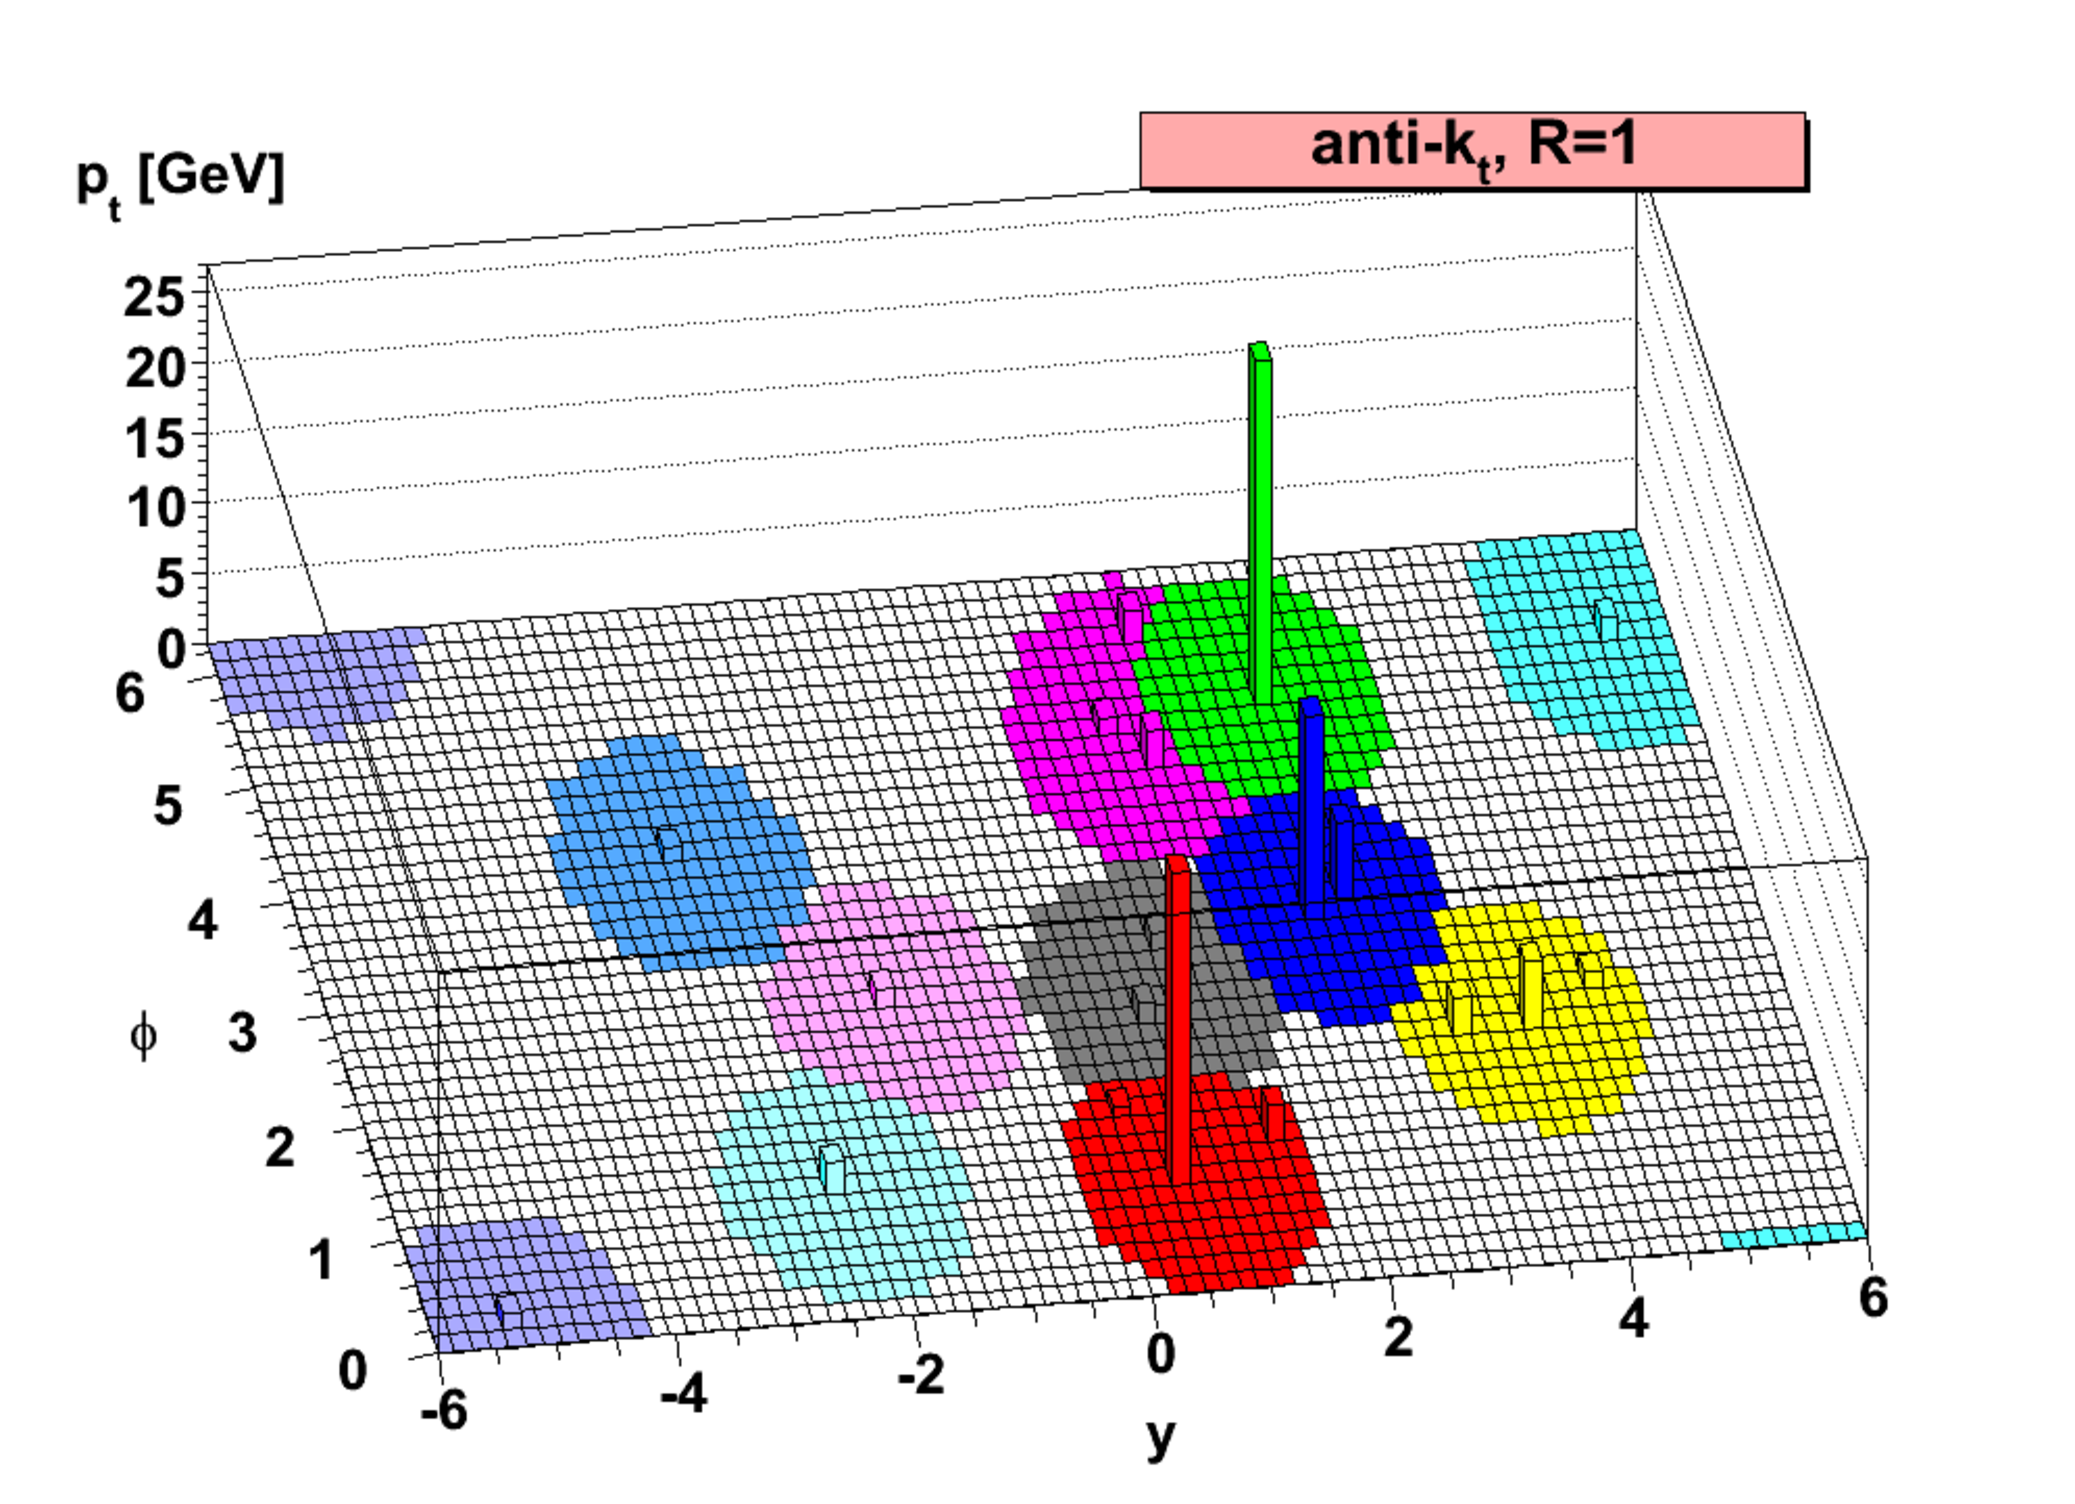
\includegraphics[width=0.4\textwidth]{ch4_figs/akt.pdf}}
    \caption{Jets in a sample MC event clustered with various algorithms.
    \label{fig:jet_cluster}}
\end{figure}

The final parameter in equation~\ref{eqn:antikt1} is defined as $R = \sqrt{\Delta\eta^{2}+\Delta\phi^{2}}$ is the conesize of the jet being clustered.
The cone size used for clustering in this analysis is R = 0.4. Versions of this analysis on 7, and 8 TeV datasets used a wider cone of 0.5. The move to smaller cone size
was motivated by the fact that jets tend to be more energetic and thus narrower and more collimated as the center-of-mass collision energy increases to 13 TeV. All techniques
mentioned above proved CMS analyzers the basic physics objects needed to perform analysis, and also standardizes the object reconstruction across the experiment. 

\section{Primary Vertex Identification and Pile-up}
Due to the way the LHC collides bunches, there are multiple pp collisions in each LHC bunch crossing at CMS. Unfortunately, many of these collisions produce
multiple objects that are reconstructed, but only 1 of these collisions is considered a hard scatter head-on collision capable of producing a \tth event.
These additional collisions that don't include the hard scatter event of interest, as well as their resulting reconstructed objects are referred to as pile-up, because
they are said to pile up on top of the objects from the collision of interest.
The collision of interest is called the primary vertex.
In this analysis and also in many others, the primary vertex is defined as the vertex with the highest \pt~sum of all constituent tracks.  
Pileup is problematic because it can make matching objects to collisions difficult. Fortunately,
CMS has an excellent tracker which makes the process of matching tracks to vertices (collision) fairly straightforward. Aside from the tracking, pileup is also
problematic because the energy deposits in the calorimeters from the pilup objects can distort the energy measurements and clustering of objects originating from
the primary vertex. There are numerous techniques to account for these effects. The technique employed in this analysis is to assign an average amount of energy
due to pileup in the detector, and subtract it off from each reconstructed jet energy measurement. This is called the rho correction.  
An example of the reconstructed tracks and vertices in an
LHC bunch crossing is below in Figure~\ref{fig:pileup_vertices}.

\begin{figure}[hbtp]
 \begin{center}
   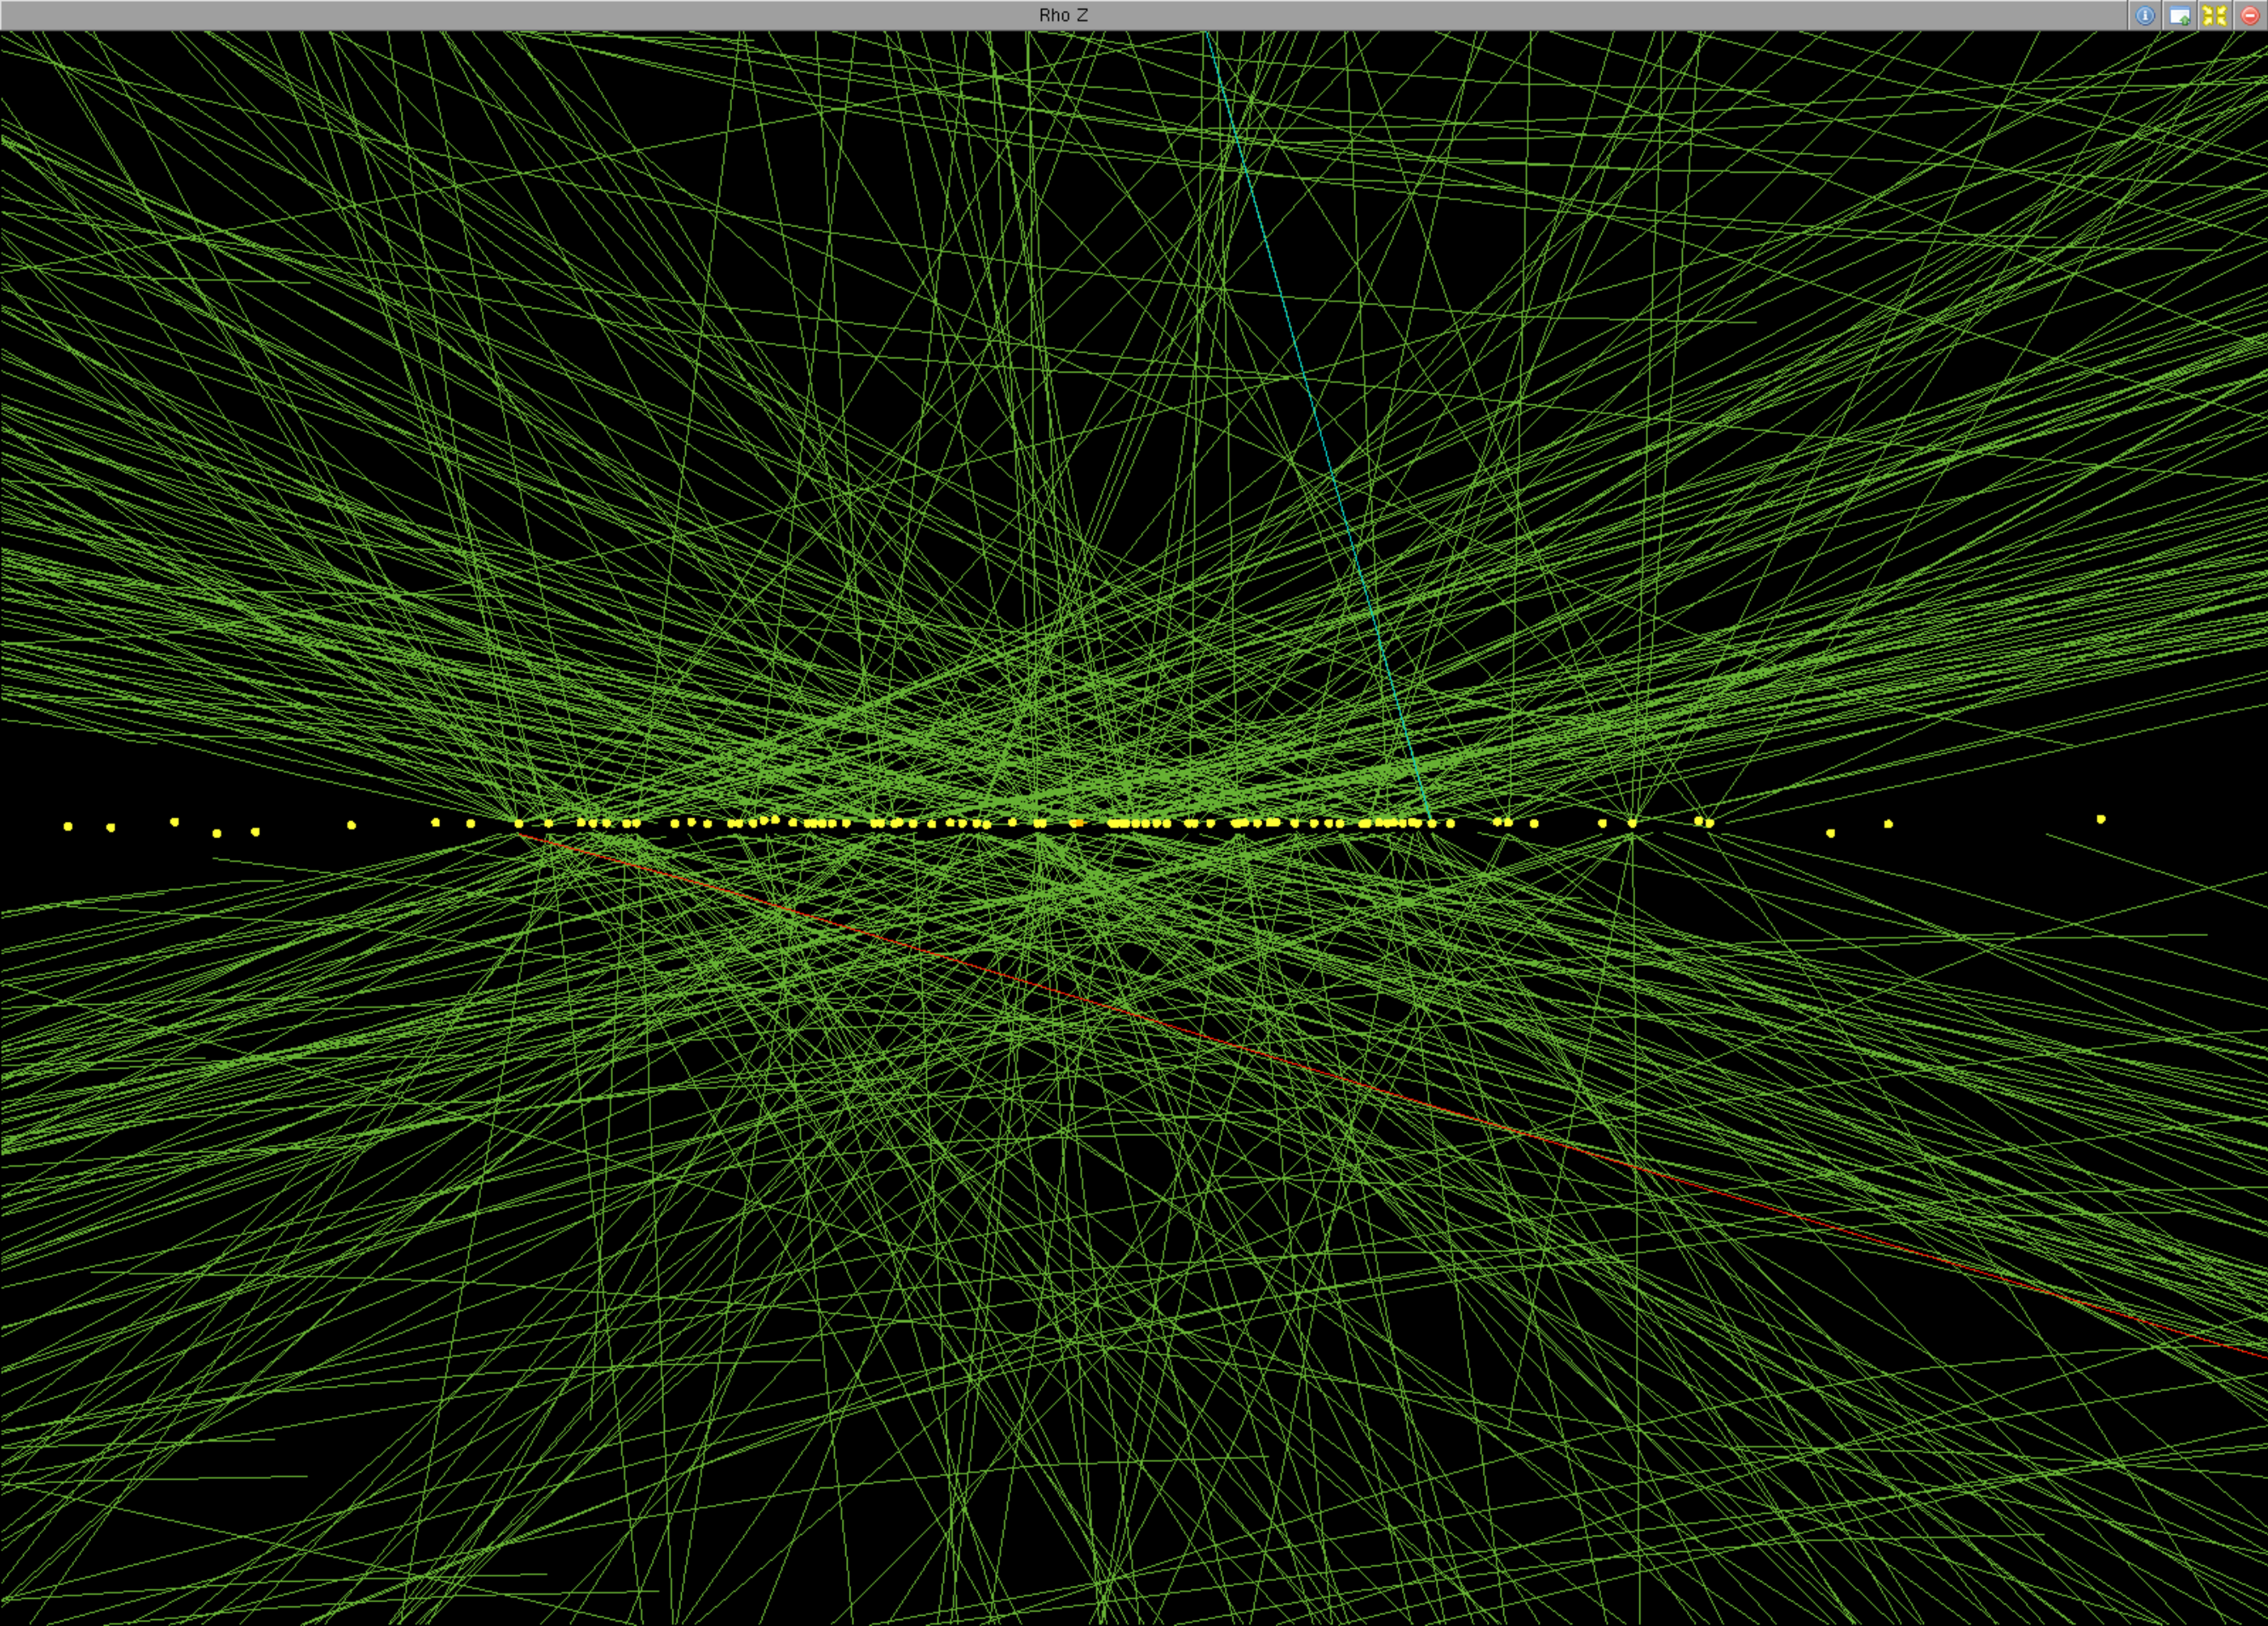
\includegraphics[width=0.8\textwidth]{ch4_figs/cms_pileup.pdf}
   \caption{A side view of the CMS tracker's reconstructed vertices in a special high pileup LHC run. The pileup in this here is 78, meaning there are
78 collisons in a single bunch crossing~\cite{pileup_image}.}
   \label{fig:pileup_vertices}
 \end{center}
\end{figure}

\noindent The pileup values in the data in this analysis varies from 30 to 45, meaning there are, on average, between 30 and 45 collisions (including the primary vertex) in each
bunch crossing recorded by CMS. 


\section{Object Selection}
After the basic object reconstruction is performed, each event is ready for the fist steps of analysis. The analysis begins with object selection where the objects in each
event are subjected to tighter criteria to ensure quality objects in the analysis that are consistent with signal and background predictions. This selection depends on and 
varies with the type of object desired in the event. Because the \tth multilepton final state is so complicated, almost\footnote{all objects except the photon, which are
used in the \tth,$H\rightarrow\gamma\gamma$ search} all objects available from the particle flow
reconstruction are needed to identify events that are consistent with the signal, namely jets, missing energy, charged leptons, and hadronic taus.

\subsection{Jets}
Jets are reconstructed from PF clusters 
\subsubsection{b-jet Identification}
\subsection{Missing Energy}
\subsection{Leptons}
\subsection{Taus}

